%sme.tex
%included in skripsie.tex

\section{Overview}
In order to test the individual system modules as well as the complete
system during its different development stages a standard measurement
environment (SME) was developed and used.The SME consists of a
physical and electrical model of the human head and emulates the
signal conditions present on the scalp surface. The use of a standard
measurement environment makes the quantitative evaluation of a
module's performance with different configurations possible. The SME
is applied as a test bench and a rapid development tool throughout the
system design cycle.


The decision to use a standard measurement environment was made in
part to circumvent logistical and safety constraints encountered while
testing system modules with human subjects:

\begin{itemize}
	\item{Protecting the subject from macro-shock conditions
	unnecessarily complicates the test procedure and system under
	investigation without any real benefit to the investigative
	process.}

	\item{The skin impedance of the subject is a function of room
	temperature and humidity. These variables may change while testing
	is in progress, obscuring parameters under observation. The
	electrode half--cell potential varies with skin pH levels and
	between electrode applications. Environmental conditions must be
	controlled to keep skin characteristics constant, complicating the
	process of system evaluation.}

	\item{The emotional condition of the subject, degree of brain
	activity, levels of stress and specifically ocular artifacts can
	complicate the testing procedure in masking unwanted internal
	noise sources with unrelated physiological signals.}
	\item{The skin potential between the stratum corneum and the
	stratum germinativum varies between individuals and is easily
	modulated by environmental conditions. This complicates the
	verification and comparison process to a large degree.}
\end{itemize}

Eliminating the need for a human signal source eases the system
development cycle and simplifies the process of evaluating the
variance of a single system parameter during a test run. 

The SME simplifies the process of testing different module
configurations while keeping external system variables constant. Using
a standard measurement environment makes it possible to vary specific
model parameters while keeping others constant. 

\section{SME design specification} \label{section:sme-design-spec}

\begin{figure}[htbp]
\begin{center}
		\psfrag{delta}{$\delta$}			
		\psfrag{theta}{$\theta$}			
		\psfrag{alpha}{$\alpha$}			
		\psfrag{beta}{$\beta$}			
		\psfrag{gamma}{$\gamma$}			
		\psfrag{Vrms}{$\mu\/V_{RMS}$}			
        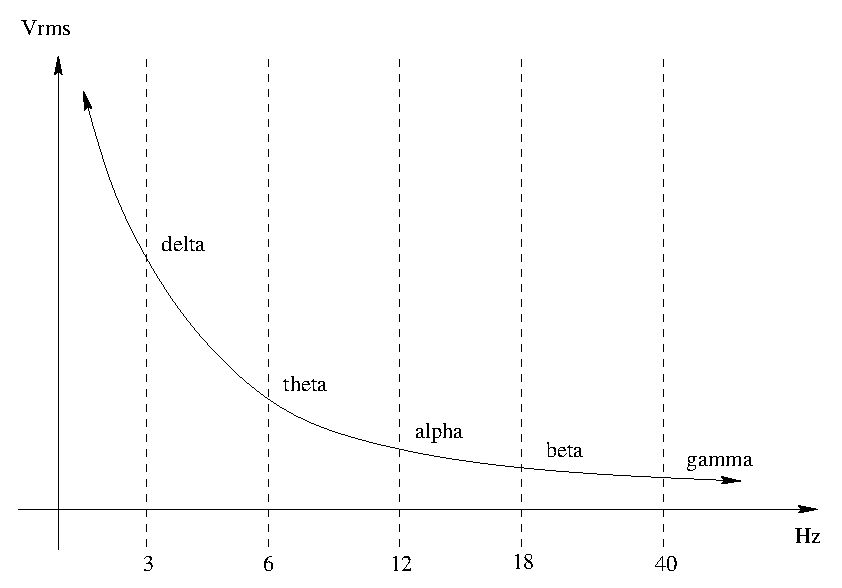
\includegraphics[width=\textwidth]{sme-eeg-power.eps}
        \caption{Simulated EEG power distribution}
        \label{fig:sme-eeg-power}
\end{center}
\end{figure}


To replace the need for a human subject the SME must be able to
accurately emulate the electrical conditions encountered on the
surface of the human scalp. Figure~\vref{fig:sme-eeg-power} depicts a
idealized EEG power spectrum as measured from various montage points
on the scalp surface. The SME's high level design specification simply
states that the SME must be able to generate a output signal having
the same power and frequency characteristics depicted in
Figure~\vref{fig:sme-eeg-power} when measured with a differential
amplifier under normal conditions. Normal conditions imply that the
amplifier has to cope with a input signal with a minimum common mode
component of 80~dB above the differential signal level.


In short: The SME must provide a output signal composed of a source
signal in the 0.1~Hz to 35~Hz band on which a +80~dB common mode
signal is superimposed. The RMS signal power levels must be within
50\% of the Figure~\ref{fig:sme-eeg-power} specification. 

In order to simplify the SME implementation and the individual
module's testing procedures only five discrete frequencies are used
for testing.

\begin{figure}[htbp]
\begin{center}
	\psfrag{eeg}[][]{$e_{EEG}$}
	\psfrag{nv}[][]{$[\mu\/V_n]$}
	\psfrag{t}[][]{time [s]}												
	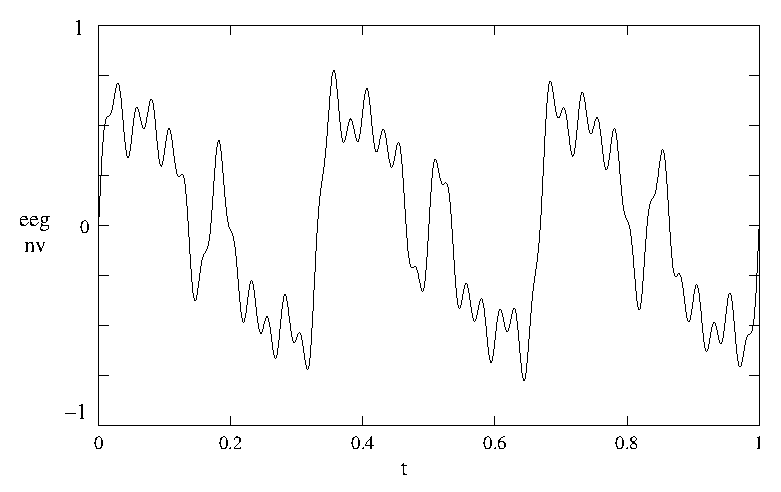
\includegraphics[width=\textwidth]{time-sim.eps}
    \caption{Simulated EEG signal.}
    \label{fig:time-sim}
\end{center}
\end{figure}

\begin{equation} \label{eq:time-sim}
	e_{EEG}(t) = \sum_{n=1}^5 A_{n}sin(f_{n}t2\pi)
\end{equation}

With $A_n$ the amplitude of the sinusoidal component $n$ and $f_n$ the
frequency of sinusoidal signal component $n$. The values of $A_n$ and
$f_n$ are listed in Table~\vref{table:test-pros}.


Figure~\vref{fig:time-sim} depicts a normalized simulated EEG signal
$e_{EEG}$ consisting of only the five frequency components noted in
Figure~\vref{fig:sme-eeg-power}. The composite signal of
Figure~\ref{fig:time-sim} is not a accurate representation of the
simulated cranial signal used during SME tests. A single frequency is
normally used for testing. Generating composite signals unnecessarily
complicates the implementation of the SME with no comparative added
functionality. The simulated signal of Figure~\vref{fig:time-sim} can
be generated by summing the outputs of the signal generators. 

Table~\vref{table:test-pros} is used during system and system module
evaluation. The $V_{pp}$ values specified is representative of the
power distribution graph depicted in Figure~\ref{fig:sme-eeg-power}.


\begin{table}
\begin{center}	
	\begin{tabular}[htpb]{|c|c|c|c|} \hline
	No. & Mark & Frequency [Hz]  & $V_{pp}$  \\ \hline
	1 & $\delta$ & 3 & 100~$\mu\/V$ \\
	2 & $\theta$ & 6 & 100~$\mu\/V$ \\
	3 & $\alpha$ & 12 & 10~$\mu\/V$ \\
	4 & $\beta$ & 18 & 20~$\mu\/V$ \\
	5 & $\gamma$ & 40 & 2~$\mu\/V$ \\
	\hline
	\end{tabular}
	\caption{SME output signal quantitative specification}
	\label{table:test-pros}
\end{center}	
\end{table}

\section{SME design and implementation}
The SME consists of a physical and electrical model of the human
head. The physical module aids in achieving the ergonomic design goals
set in section~\vref{section:def-of-need}. The physical model also
serves as a test bed for evaluating variations in the signal
acquisition module's container design. A electrical model is
implemented using sinusoidal and noise signal generators. The SME
presents a model signal to the signal acquisition module incorporating
the main characteristics of a natural cranial surface signal.

\subsection{SME Physical model}

\begin{figure}[htbp]
\begin{center}
	\psfrag{Base strips}[][]{Base strips}
	\psfrag{Head model}[][]{Head Model}
	\psfrag{Electrode contacts}{Electrode contacts}	
	\psfrag{Common mode }[][]{Common mode}							
	\psfrag{and signal}[][]{and signal }
	\psfrag{source}[][]{source}
	\psfrag{EM shielding}[][]{EM Shielding}
	\psfrag{SA }{SA }
	\psfrag{Module}{Module }
	\psfrag{Container}[][]{Container}
	\psfrag{fp1}[][]{$F_{p1}$}				
	\psfrag{fp2}[][]{$F_{p2}$}
	\psfrag{ref}[][]{$ref$}	
	\psfrag{ec}[][]{ ($e_c$)}		
	\psfrag{eb}[][]{ ($e_b$)}												
    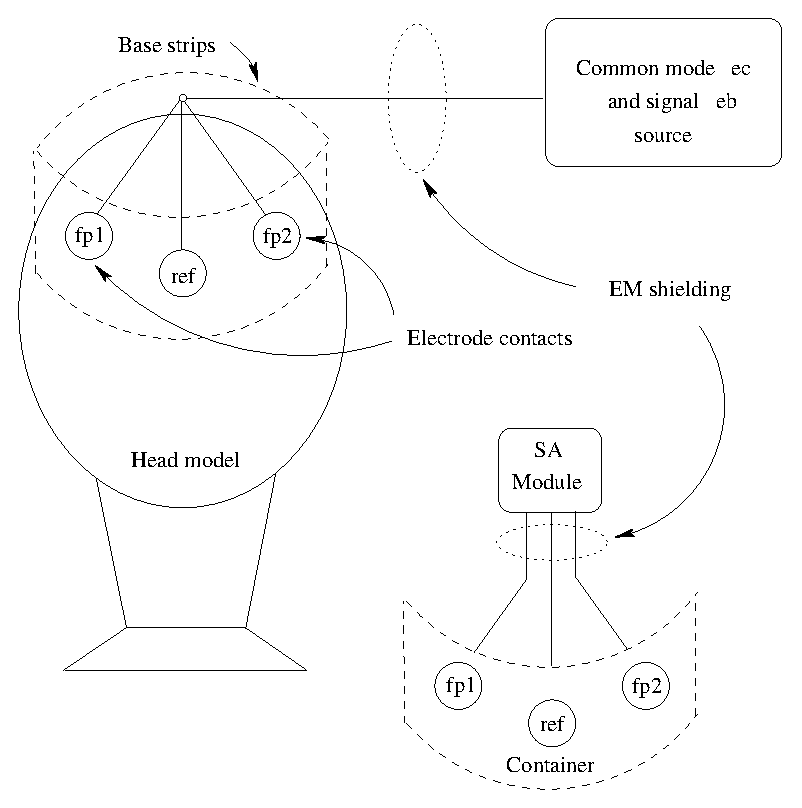
\includegraphics[width=\textwidth]{standard-measurement-environment.eps}
    \caption{Physical model of the standard measurement environment.}
    \label{fig:standard-measurement-environment}
\end{center}
\end{figure}


Figure~\vref{fig:standard-measurement-environment} is a diagram of the
physical model of the SME. The SME module is constructed using a
standard polystyrene hat--fitter head model. These models are widely
available and easily replaceable. The polystyrene model is painted to
provide a extra protective layer against the wear and tear of
laboratory use.  Horizontal and vertical foam rubber strips are glued
onto the painted surface to assist in the physical fitting of the
container. Electrical contacts are fastened to the surface rubber
strips at the $F_{p1}$ and $F_{p2}$ locations as defined by the 10--20
EEG montage protocol
\cite[p3-4]{eeghand}. Accurately establishing the physical distance
between the electrodes on the SME ensures that the signal acquisition
module (SAM) takes the possible detrimental effect of interference
from lead wires into account. The electrode contacts are connected to
the signal generators $e_b$ and $e_c$
(Figure~\ref{fig:standard-measurement-environment}) via 5~cm lengths
of shielded wiring. The signal generators are mounted close to the
electrical contacts on the rear side of the head model, see
Figure~\vref{fig:sme-photo}.


The removable SAM--container is mounted on top of the base strip with
the electrodes touching the electrical contacts. This arrangement
enables the worker to easily test and calibrate the various modules
and the complete system, while keeping the physical and electrical
model parameters constant. The container hosts the signal acquisition
module electronics and does not logically fit with the SME. The
container is depicted with
Figure~\ref{fig:standard-measurement-environment} to illustrate the
physical fit between the SME and the signal acquisition module while
testing the various system modules.

\begin{figure}[htbp]
\begin{center}
	%\vspace{8cm}
	\includegraphics*{sme-head.eps2}
	\caption{SME Photograph}
\label{fig:sme-photo}
\end{center}
\end{figure}

Figure~\ref{fig:sme-photo} is a photograph of the SME module used
during testing and development. The electrical contacts can be seen at
the $F_{p1}$ and $F_{p2}$ positions. The signal generators are
mounted to the rear of the model below the inion. The Signal
Acquisition module's container is fastened on top of the the SME with
the electrodes aligned over the electrical contacts using Velcro
strips.



\subsection{SME Electrical model}
\begin{figure}[ht]
\begin{center}
	\psfrag{Head}{Head}
	\psfrag{A}{A}
	\psfrag{B}{B}
	\psfrag{re}{$r_e$}		
	\psfrag{rc}{$r_c$}		
	\psfrag{eb}[][]{$e_b$}		
	\psfrag{ec}[][]{$e_c$} %common signal across dif inputs 		
	\psfrag{Eeeg}[][]{\colorbox{white}{$e_{EEG}$}}			
	\psfrag{r1}{$R_{s1}$}
	\psfrag{r2}{$R_{s2}$}				
	\psfrag{c1}{$C_1$}		
	\psfrag{c2}{$C_2$}		
	\psfrag{O1}{$O_1$}		
	\psfrag{O2}{$O_2$}		
	\psfrag{O3}{$ref$}		
	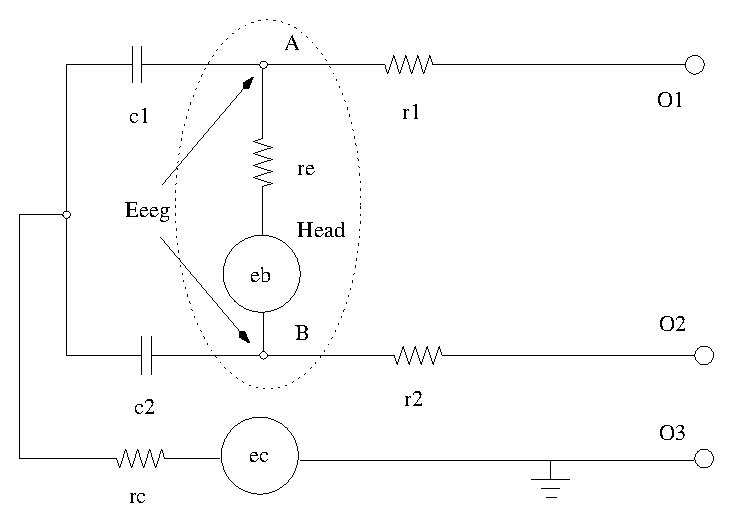
\includegraphics[width=\textwidth]{sme-eq.eps}
	\caption{Electrical model of the standard measurement environment.}
	\label{fig:sme-eq}
	\end{center}
\end{figure}

The SME must be able to emulate the electrical behavior normally
measured on the scalp surface for experimental and modeling
purposes. The brain is the source of the electrical activity measured
as the EEG signal. The dry skin surface as well as the underlying soft
tissue acts as volume conductors from the signal source to the
electrode surfaces. The conduction pathways tend to act as low--pass
signal filters attenuating the signal. This behavior is simulated with
a resistive circuit that lumps the various skin impedances together.

Figure~\vref{fig:sme-eq} summarizes the electrical model implemented
by the SME.
\begin{itemize}

	\item{Outputs $O_1$ and $O_2$ represent the SME output
	signals. The $ref$ label represents the SME signal ground
	reference. The output signals and signal ground are accessible
	through electrical contacts mounted on the SME physical model, see
	Figure~\vref{fig:standard-measurement-environment}.}


	\item{The $R_{s1}$ and $R_{22}$ values are the equivalent scalp
	resistances. $R_{s1} = R_{s2} = 10~k\Omega$
	\cite{intro-to-bio}.}

	\item{The $e_b$ signal is the Th\`{e}venin equivalent voltage
	source as seen by the electrodes (A-B). The $e_b$ voltage is the
	representation of all electrical activity volume conducted to a
	central point between electrodes. This signal is chosen from the
	options available in Table~\ref{table:test-pros} depending on
	module being developed or tested. The 12~Hz $\alpha$ signal were
	used most frequently as it lies fairly central in the EEG band of
	interest.}

	\item{The $r_e$ value is the Th\`{e}venin equivalent resistance of
	the signal source as seen by the electrodes (A-B). The $r_e$ value
	was chosen as 10~k$\Omega$, \cite{intro-to-bio}.}

	\item{Common source signal $e_c$ is capacitively coupled through
	$C_1$ and $C_2$ into $O_1$ and $O_2$. The common-mode voltage
	$e_c$ simulates all interference signal sources attributable to
	50~Hz power--line noise, power equipment and fluorescent lights
	\cite{fluorescent-interference},
	\cite{fluorescent-interference2}. The values of $C_1$ and $C_2$
	was chosen as 2pF, \cite{drive}, and $r_e = 10~k\Omega$.}
\end{itemize}

The EEG signal $e_{EEG}$ is generated using a approximately 100~$\mu$V
sinusoidal signal source. Common mode voltage $e_c$ is the sum of two
large amplitude signals, a sinusoidal signal $e_{cs}$ (1--100~mV) and
a white noise signal $e_{white}$ with amplitude range
1~mV$_{rms}$--100~mV$_{rms}$. The white noise signal ($e_{white}$) is
used during bandwidth tests and can be coupled in and out of the
SME. The common mode voltage $e_c$ is added to $e_{EEG}$ via $C_1$ and
$C_2$. A differential measurement between $O_1$ and $O_2$ with respect
to $ref$ yields a signal similar to $e_{EEG}$.

Although this model of electrical scalp activity is rather contrived
it adequately serves the purpose for which it was designed.

\subsubsection{Interference reduction}
In order to eliminate external interference the complete SME
environment is housed in a rectangular 100X150X50~cm metal box acting
as a Faraday cage. The cage is manufactured from plate metal and
square tubing. The cage interior is accessed via a hinged hatch,
forming one of the cage walls when shut.

The SME is electrically accessed via a set of 2~mm female RCA jacks
and is internally powered from a set of re-chargeable 9~V
nickel--cadmium batteries. Electrically isolating the whole SME
environment allows for the rapid prototyping of system modules without
the added complexity of uncontrolled signal contamination due to
external interference.

The rest of this chapter is dedicated to the implementation details of
the signal generators used in generating $e_c$ and $e_{EEG}$.


\subsection{Signal generation overview}
\label{section:sin}
Two distinct signal types are used in the SME -- sinusoidal signals
and white noise. The generators used to create $e_{EEG}$ and the
sinusoidal component of $e_c$ differ only in the signal output
amplitude and frequency. The same basic circuit is used to implement
all sinusoidal signal generators in the SME. The common mode signal
$e_c$ has a white noise component $c_{white}$ used during noise
suppression and filter bandwidth tests. The $c_{white}$ circuit is
implemented using a zener diode as noise source.


The common mode signal $e_c$ is the sum of a sinusoidal ($e_{cs}$) and
a white noise ($e_{white}$) signal. Separate signal generators are
used to create the $e_{white}$ and $e_{cs}$ components of $e_c$. The
common mode signal is summed with $e_{EEG}$ via the couple
capacitances $C_1$ and $C_2$ of Figure~\ref{fig:sme-eq}. The
amplitude and bandwidth variable common mode signal source is used to
evaluate a module's dynamic response as well as the common mode
rejection ratio of the low level signal processing module.


The various filters used throughout the system is tested by adjusting
the frequency of $e_c$ beyond the evaluated filter's cut--off point,
and measuring the resulting output signal. Because EEG signals,
external interference and internal system generated noise are all
inherently stochastic by nature this approach is considered to be a
good emulation of normal system behavior.

\subsection{Sinusoidal signal generation - $e_b$ and $e_{cs}$} 
\label{section:wein}
\subsubsection{Overview}
The SME electrical model makes use of sinusoidal signal generators as
both common--mode ($e_c$) and differential--mode ($e_b$) signal
sources. A common Wein--bridge circuit design \cite[p30-32]{analog}
\cite[p344-349]{master} \cite[p296-297]{art} 
is used in implementing all the sinusoidal signal generators used in
the SME. The specific component values are varied to achieve desired
frequency and amplitude specifications.

\subsubsection{Design specification}
The sinusoidal signal generators used in the SME are required to be
exceptionally pure and stable. A test signal must have a internal
distortion factor at least ten times smaller than the expected system
distortion levels to establish a accurate representation of the system
distortion, \cite[p296]{art}. A stable oscillator design with maximum
residual distortion of less than 0.05\% is called for.

\subsubsection{Implementation}
\begin{figure}[htbp]
\begin{center}
	\psfrag{+}{+}
	\psfrag{-}{--}
	\psfrag{a}{$a$}
	\psfrag{b}{$b$}
	\psfrag{r}{$R$}
	\psfrag{c}{$C$}
	\psfrag{rf}{$R_{fb}$}
	\psfrag{ira}{$i_{R_{ad}}$}
	\psfrag{ra}{$R_{ad}$}
	\psfrag{vsin}{$e_{sin}$}
	\psfrag{TL071}[][]{071}
	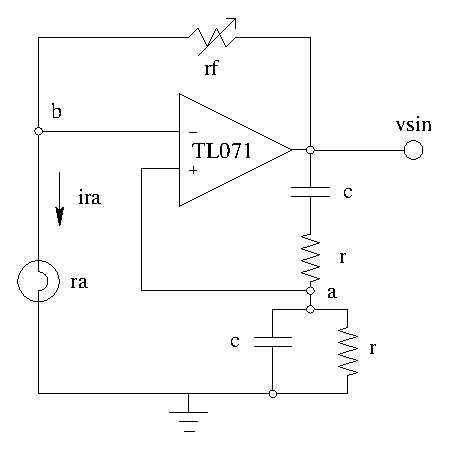
\includegraphics{sin-source.eps}
    \caption{Sinusoidal signal generator.}
    \label{fig:sin-source}
\end{center}
\end{figure}

Wein--bridge oscillators are known for their exceptional stability and
low distortion at low frequencies. The signal generator of
Figure~\ref{fig:sin-source} consists of an operational amplifier with
two complex impedances in its positive feedback path forming one tier
of the bridge. The circuit operates in non-inverting mode with the
non-inverting input signal $v_a$ created by the voltage divider at
node $a$. The negative feedback path consists of two real impedances
controlling circuit gain. $R_{ad}$ is a filament lamp with resistance
inversely proportionate to current.



\subsubsection{Circuit analysis}
The circuit analysis of the circuit in Figure~\vref{fig:sin-source} is
done by equating the real and imaginary components of $v_a$ and $v_b$,
\cite[p31]{analog}.

The impedance of the series $RC$ network is:
\begin{equation}
	Z_{s} = \frac{1 + sRC}{sC}
	\label{eq:zs}
\end{equation}

The impedance of the parallel $RC$ network is:
\begin{equation}
	Z_{p} = \frac{R}{1 + sRC}
	\label{eq:zp}
\end{equation}

At node $a$, the non-inverting amplifier input, the voltage $v_a$ is
determined by the voltage divider formed by $Z_{s}$ and $Z_{p}$:
\begin{equation}
	v_{a} = \frac{e_{sin}RCs}{R^2C^2s^2 + 3RCs + 1}
	\label{eq:va}
\end{equation}

At node $b$, the inverting amplifier input, the voltage $v_b$ is
determined by the voltage divider formed by $R_{fb}$ and $R_{ad}$:
\begin{equation}
	v_{b} = \frac{e_{sin}}{1 + \frac{R_{fb}}{R_{ad}}}
	\label{eq:vb}
\end{equation}

The operational amplifier adjusts $e_{sin}$ to equate $v_a$ and $v_b$
via the positive and negative feedback loops, from the amplifier
action follows that:
\begin{equation}
	\frac{RCs}{R^2C^2s^2 + 3RCs + 1} = \frac{1}{1 + \frac{R_{fb}}{R_{ad}}}
	\label{eq:va=vb}
\end{equation}

For a constant $e_{sin}$ output amplitude $\sigma$ is set to zero in
$s = \sigma +j\omega$.  Substituting $s = j\omega$ in
Equation~\ref{eq:va=vb} and grouping real and imaginary terms yields
Equation~\ref{eq:va=vb} in terms of $\omega$:
\begin{equation}
	\frac{-\omega\/RC}{j(1 - \omega^2R^2C^2) - 3\omega\/RC} =
	\frac{1}{1 + \frac{R_{fb}}{R_{ad}}} 
	\label{eq:va=vbj}
\end{equation}

Equating imaginary terms on both sides of Equation~\ref{eq:va=vbj}
yields the equation for calculating the frequency of the output signal
$e_{sin}$.
\begin{equation}
	1 - \omega\/^2R^2C^2 = 0
	\rightarrow f = \frac{1}{2\pi\/RC}
	\label{eq:f}
\end{equation}

Equating real terms on both sides of Equation~\ref{eq:va=vbj} yields
the relationship between $R_{fb}$ and $R_{ad}$:
\begin{equation}
	R_{fb} = 2R_{ad}
	\label{eq:r}
\end{equation}

Substituting $R_{fb} = 2R_{ad}$ in Equation~\ref{eq:vb} and solving
for $\frac{e_{sin}}{v_b}$ yields a circuit gain $G = 3$. $R_{ad}$
varies with the current ($i_{R_{ad}}$)flowing through it stabilizing
the system gain. If $G < 3$ more energy is lost than being added and
oscillations die out, if $G > 3$ the amplifier saturates and $e_{sin}$
converges to one of the supply rail voltages. The feedback resistance
$R_{fb}$ is adjusted to 2$R_{ad}$, when $e_{sin}$ decreases the
$i_{R_{ad}}$ current through $R_{ad}$ decreases causing $R_{ad}$'s
temperature to drop. A decrease in $R_{ad}$ temperature lowers its
resistance which causes the circuit gain and consequently $e_{sin}$ to
increase proportionately. This cyclic behavior is governed by the
large time constant gain setting feedback introduced by $R_{ad}$.

Using Equations~\ref{eq:f} and \ref{eq:r} circuit component values can
be computed to satisfy the requirements of each sinusoidal signal
generator needed in the SME.

\begin{figure}[htbp]
	\begin{center}
	\psfrag{r}{$R$}
	\psfrag{f}{$f$}
	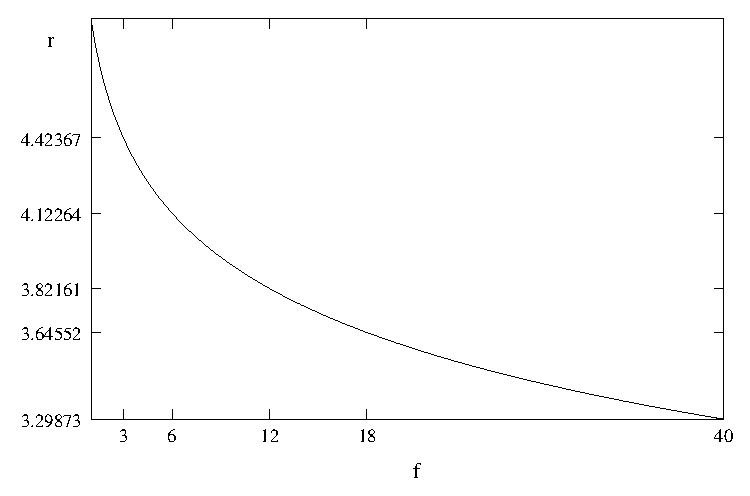
\includegraphics[width=\textwidth]{sin-r.eps}
    \caption{Resistance--Frequency (C=2~$\mu$F)}
    \label{fig:sin-r}
	\end{center}
\end{figure}

Figure~\vref{fig:sin-r} plots $R = log_{10}(\frac{1}{2\pi\/RC})$ for a
chosen capacitance $C = 2\mu$F. From Figure~\vref{fig:sin-r}
approximate resistance values are chosen, these are listed in
Table~\vref{table:r-c}. The precision of the quoted values does not
reflect the accuracy of the resistances used in the generator
implementation. Although 1\% resistances were used throughout the
design, values can only be chosen from a fixed set. Where appropriate
resistances were corrected using series or parallel combinations.


\begin{table}
\begin{center}	
	\begin{tabular}[htpb]{|c|c|l|l|} \hline
	No. & Mark & Frequency [Hz]  & $R$  \\ \hline
	1 & $\delta$ & 3 & 26.5~k$\Omega$ \\
	2 & $\theta$ & 6 & 13.3~k$\Omega$ \\
	3 & $\alpha$ & 12 & 6.7~k$\Omega$ \\
	4 & $\beta$ & 18 & 4.4~k$\Omega$ \\
	5 & $\gamma$ & 40 & 2.0~k$\Omega$ \\
	\hline
	\end{tabular}
	\caption{Resistance values for $C=2~\mu\/F$}
	\label{table:r-c}
\end{center}	
\end{table}

All resistances are 1\% accurate metal--film devices with good
temperature stability. Polypropylene capacitors are used because of
their good accuracy, temperature stability and low leakage properties,
\cite[p22]{art}.


\subsection{Noise generation - $e_{white}$}
\label{section:noise}
\subsubsection{Overview}
This section details the design and implementation of the noise
generator used in the standard measurement environment. The noise
source $e_{white}$ is applied capacitively to both electrodes and is a
component of the common--mode signal as seen by the differential
inputs of the low level signal processing module.


\subsubsection{Design specification}
The noise generator must be capable of generating a relatively flat
spectrum white noise signal in the 0.1~Hz to 200~Hz range. White noise
is defined as having equal power per Hz, the noise generator only
needs to approximate a white noise source in the operative bandwidth.


\subsubsection{Implementation}
The noise generator is implemented using analog electronic circuitry
based on the avalanche noise generated by a reverse biased zener
diode. Avalanche noise is created when a PN junction is operated in
reverse breakdown mode \cite[p3]{noise-analysis}. Electrons accelerate
in the reverse electric field within the PN junction depletion zone
gathering enough kinetic energy to dislodge other electrons from the
atoms in the junction crystal lattice.

Good quality low--voltage zener diodes are not readily available
commercially and an alternative device is used instead.

The LM336 device simulates a low voltage zener diode and is ideally
suited for analogue noise generator applications. The low device
voltage supports long battery life in operation. The LM336 may be
operated over a wide voltage range which further extends the usable
battery life. The device noise specification is available from the
product specification sheet. The frequency response noted in the
product sheet is a valuable yardstick when evaluating the individual
module frequency responses. The frequency response of each module is
compared with the LM336 product sheet noise specification and must
correlate to a high degree for an adequately designed and implemented
module.

\begin{figure}[htbp]
	\begin{center}
	\psfrag{1}{1}
	\psfrag{2}{2}
	\psfrag{3}{3}
	\psfrag{8}{8}
	\psfrag{r1}{$R_1$}
	\psfrag{r2}{$R_2$}
	\psfrag{r3}{$R_3$}
	\psfrag{c1}[][]{\colorbox{white}{$C_1$}}	
	\psfrag{c2}[][]{\colorbox{white}{$C_2$}}	
	\psfrag{c3}{$C_3$}
	\psfrag{c4}{$C_4$}
	\psfrag{c5}[][]{$C_5$}
	\psfrag{c6}{$C_6$}
	\psfrag{c7}{$C_7$}
	\psfrag{ew}{$e_{white}$}
	\psfrag{+}{+}		
	\psfrag{-}{--}
	\psfrag{+9V}{+9 V}
	\psfrag{LM336}[][]{LM336}				
	\psfrag{386}[][]{386}				
	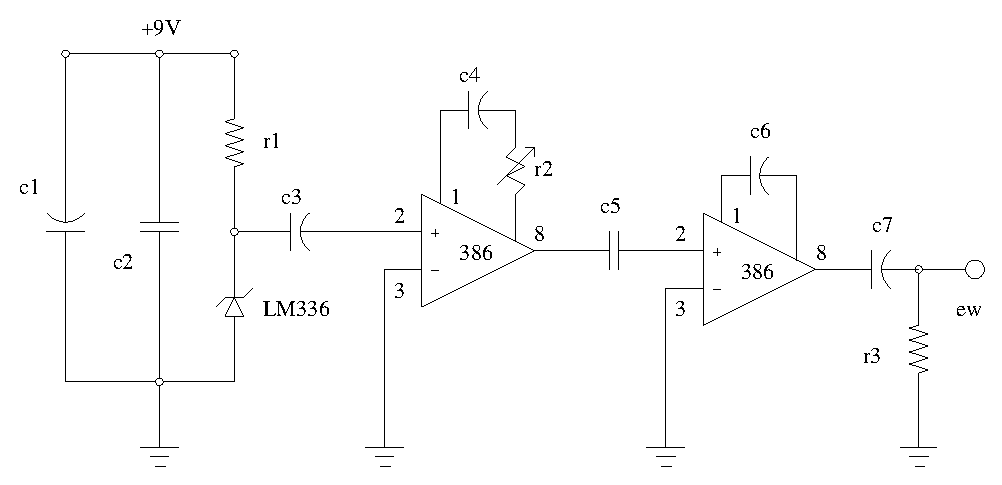
\includegraphics[width=\textwidth]{noise-generator.eps}
    \caption{White noise generator.}
    \label{fig:noise-generator}
	\end{center}
\end{figure}

Fig~\vref{fig:noise-generator} depicts the circuit diagram of the SME
white noise generator circuit. The circuit amplifies the zener noise
voltage from the LM336 through two LM386 cascaded amplifiers. The
second amplifier is used for calibration purposes and usually
disabled. Each LM386 nominally contributes 26~dB gain. The 10~$\mu$F
capacitors between pins 1 and 8 sets the amplifier gain to 200 or
46~dB if the variable resistor is set to 0~$\Omega$. The variable
resistor adjusts the amplifier gain between 20 and 200. Gain control
can also be done by capacitively coupling a resistor or FET from pin 1
to ground.

Additional external components can be placed in parallel with the
device's internal feedback resistors to adjust the frequency and gain
response. This technique is applied to band--limit the output of the
noise generator to 500Hz. 

\begin{table}
\begin{center}	
	\begin{tabular}[htpb]{|l|l|} \hline
	$C_1$ & 0.01~$\mu$F \\
	$C_2$ & 100~$\mu$F \\
	$C_3$ & 0.47~$\mu$F \\
	$C_4$ & 10~$\mu$F \\
	$C_5$ & 0.01~$\mu$F \\
	$C_6$ & 10~$\mu$F \\
	$C_7$ & 15~$\mu$F \\
	$R_1$ & 15~k$\Omega$ \\
	$R_2$ & 0~--~20~k$\Omega$ \\
	$R_3$ & 24~k$\Omega$ \\
	\hline
	\end{tabular}
	\caption{White noise generator component values}
	\label{table:noise-val}
\end{center}	
\end{table}

Table~\vref{table:noise-val} summarizes the component values used in
the white noise generator implementation.


\section{$e_{EEG}$ integration}

The $e_{EEG}$ signal of Figure~\vref{fig:sme-eq} is the output of a
sinusoidal signal source $e_{b}$ and a series resistance $r_e$.

\begin{figure}[htbp]
	\begin{center}
	\psfrag{a}{$\alpha$}
	\psfrag{th}{$\beta$}
	\psfrag{r}{$R_{\alpha}$}
	\psfrag{c}{$C$}
	\psfrag{c2}{$C$}
	\psfrag{r2}{$R_{\beta}$}
	\psfrag{eeeg}{$e_{EEG}$}
	\psfrag{ra}{$lamp$}
	\psfrag{rf}{$trim$}
	\psfrag{re}{$R_l$}
	\psfrag{rl}{$R_e$}
	\psfrag{TL071}[][]{071}
	\psfrag{+}{+}
	\psfrag{-}{--}
	\psfrag{+}{+}
	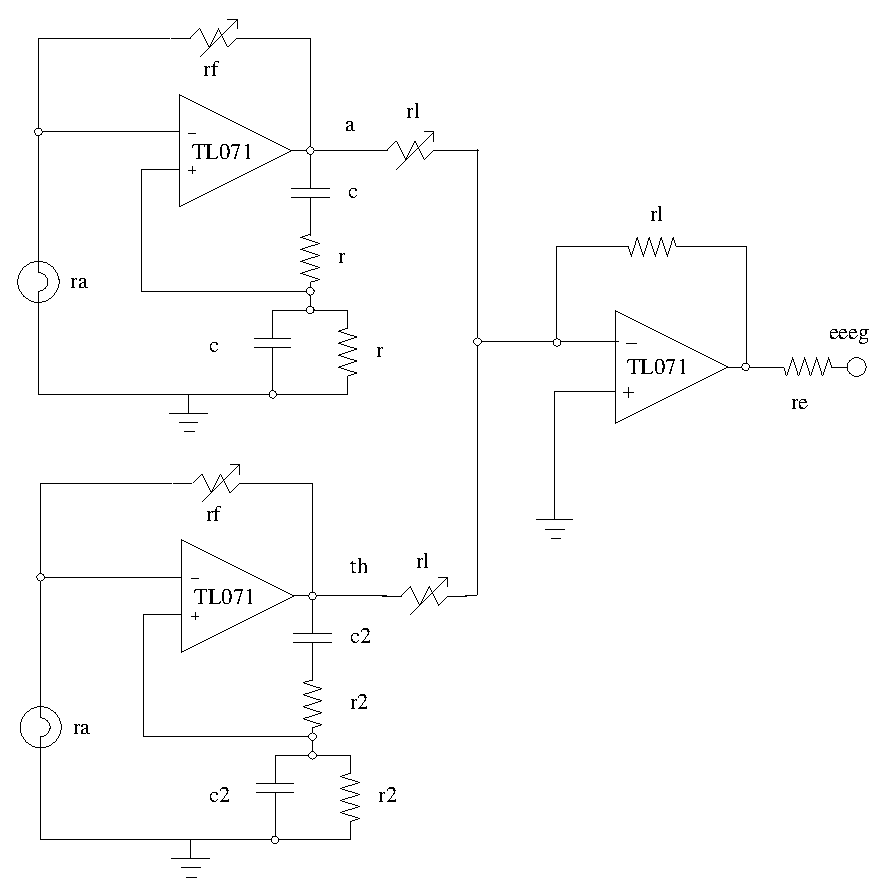
\includegraphics[width=\textwidth]{eeeg.eps}
    \caption{$e_{EEG}$ integration.}
    \label{fig:eeeg}
	\end{center}
\end{figure}

Figure~\vref{fig:eeeg} illustrates how $e_b$ is implemented using one
or more of the Wein--bridge oscillators described in
Section~\ref{section:sin}. In Figure~\vref{fig:eeeg} only the $\alpha$
and $\beta$ signals are summed to produce $e_{EEG}$. The $e_{EEG}$
signal is the sum of the voltages $\alpha$ and $\beta$ weighted by the
reciprocals of their input resistance values. By varying the input
resistors the contribution of each input signal to $e_{EEG}$ is
changed to reflect the signal voltage values specified in
Table~\vref{table:test-pros}.



The $e_{EEG}$ signal has a very low output impedance as can be
expected from the operational amplifier output stage of the adder
circuit. A 10~k$\Omega$ series resistance $r_e$ is added in order to
emulate the cranial impedance of a real human head. The addition of
$r_e$ makes it possible to use the SME as a general test bench. 

The purely resistive model of cranial impedance ($r_e$) used in the
SME is considered to be adequate for the bandwidth under
investigation. Phase errors and reactive impedance introduced by the
skin is considered small enough to be neglected. The SME can therefore
not be used for high--frequency skin or bone impedance measurements.

\begin{table}
\begin{center}	
	\begin{tabular}[htpb]{|l|l|} \hline
	$C$ & 2~$\mu$F \\
	$R_{\alpha}$ & 6.7~k$\Omega$ \\
	$R_{\beta}$ & 4.4~k$\Omega$ \\
	$R_e$ & 10~k$\Omega$ \\
	$R_l$ & 10~k$\Omega$ \\
	$trim$ & 0 -- 1~k$\Omega$ \\
	\hline
	\end{tabular}
	\caption{$e_{EEG}$ generator component values}
	\label{table:eeg-val}
\end{center}	
\end{table}

Table~\vref{table:eeg-val} summarizes the component values used in the
$e_{EEG}$ generator implementation.


\section{$e_c$ integration}
\begin{figure}[htbp]
	\begin{center}
	\psfrag{rf}{$trim$}
	\psfrag{r}{$R_{50Hz}$}
	\psfrag{rl}{$R_l$}
	\psfrag{r2}{$R_2$}
	\psfrag{c}{$C$}
	\psfrag{int}{$e_{cs}$}
	\psfrag{ecn}{$e_{s}$}	
	\psfrag{ew}{$e_{white}$}
	\psfrag{ec}{$e_c$}
	\psfrag{ra}{$lamp$}
	\psfrag{TL071}[][]{071}
	\psfrag{+}{+}
	\psfrag{-}{--}
	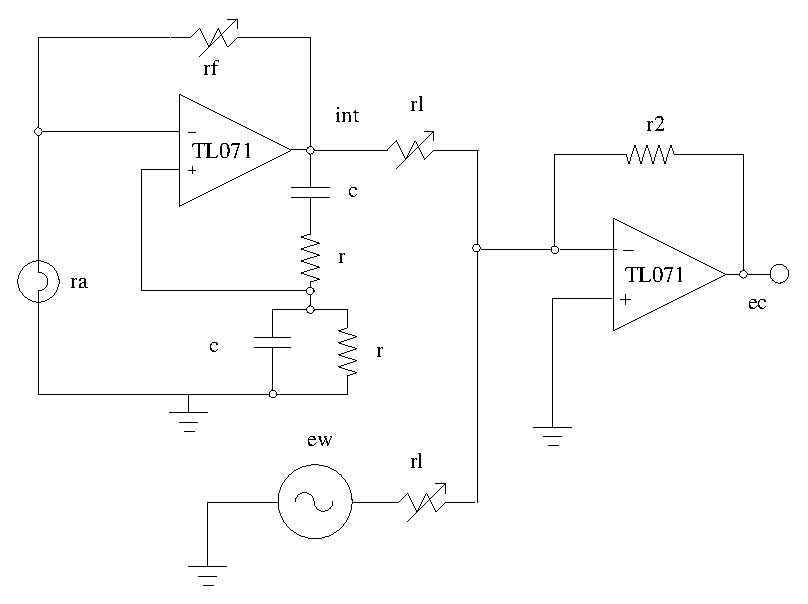
\includegraphics[width=\textwidth]{ec-int.eps}
    \caption{$e_c(t) = e_{sn} + e_{white}$.}
    \label{fig:ec-int}
	\end{center}
\end{figure}

The common mode signal $e_c$ is the sum of the sinusoidal signal
$e_{ns}$ and the white noise signal $e_{white}$. $e_{ns}$ is
implemented using the Wein-bridge circuit of
Section~\ref{section:wein} on page \pageref{section:wein}. The
$e_{cs}$ signal represents power line interference, the circuit of
Figure~\vref{fig:ec-int} oscillates at 50~Hz for the given resistance
value of 1.6~k$\Omega$.  $e_{white}$ is implemented using the circuit
described in Section~\ref{section:noise}.

The noise signal $e_{white}$ is added to $e_{ns}$ using the standard
operational amplifier summing circuit of Figure~\vref{fig:ec-int}. The
$R_l$ input resistances (0--20~k$\Omega$) is varied to adjust the
contribution of $e_{white}$ and $e_{cs}$ to the common mode signal
$e_c$.

\begin{table}
\begin{center}	
	\begin{tabular}[htpb]{|l|l|} \hline
	$C$ & 2~$\mu$F \\
	$R_{50Hz}$ & 1.6~k$\Omega$ \\
	$R_2$ & 10~k$\Omega$ \\
	$R_l$ & 0 -- 20~k$\Omega$ \\
	$trim$ & 0 -- 1~k$\Omega$ \\
	\hline
	\end{tabular}
	\caption{$e_c$ generator component values}
	\label{table:ec-val}
\end{center}	
\end{table}

Table~\vref{table:ec-val} summarizes the component values used in the
$e_c$ generator implementation.



\section{SME simulation}
The various signal sources used in the SME implementation are
simulated in order to facilitate the visual inspection of generator
outputs. As all signals in the SME are linearly summed it is necessary
to ensure that composite signal amplitudes does not drive the various
active components into non--linear regions distorting the test
signal. Source signal amplitudes are adjusted to ensure a linear SME
signal source. The signal simulations are used to accurately predict
and set maximum signal amplitudes.

\subsection{$e_b$ simulation}

\begin{figure}[htbp]
\begin{center}
	\psfrag{t}{time [s]}
	\psfrag{eb}[][]{$e_b$ [$\mu$V]}
	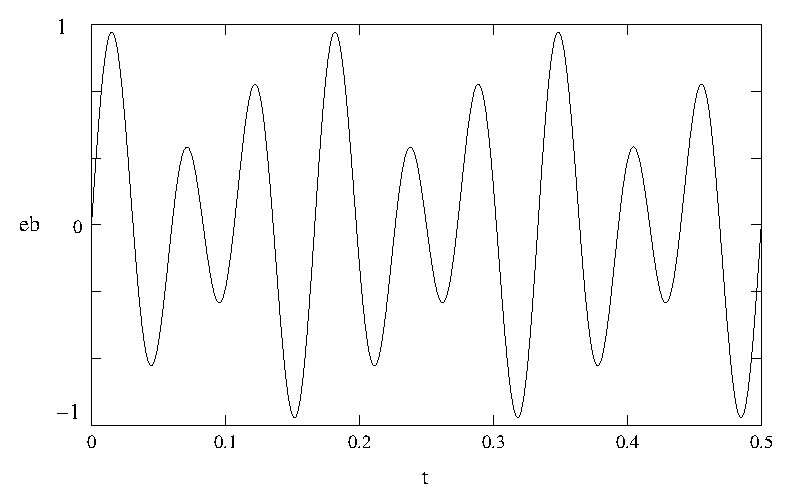
\includegraphics[width=\textwidth]{eb-sim.eps}
    \caption{$e_b(t)_{\alpha + \beta}$ simulation.}
    \label{fig:eb-sim}
\end{center}
\end{figure}

Figure~\vref{fig:eb-sim} depicts the normalized output of the
composite $e_b$ signal source set at the specified $\alpha$ and
$\beta$ frequencies.

\begin{equation} \label{eq:theta-sim}
	e_b(t)_{\alpha + \beta} = A_{\alpha}\sin\/(2\pi\alpha\/t) +
	A_{\beta}\sin\/(2\pi\beta\/t)
\end{equation}

$A_{\alpha}$ and $A_{\beta}$ are specified in
Table~\vref{table:test-pros}.

The power spectrum of Figure~\vref{fig:sme-eeg-power} is a averaged
signal and does not reflect the instantaneous power of a frequency
component. It is however prudent to note that the S/N ratio of the
$\gamma$ signal (40~Hz) is very low as the average amplitude of a
$\gamma$ band signal is $<2\mu\/V$. It would therefore be inaccurate
to use a high amplitude $\gamma$ frequency signal as a standard SME
test signal.


\subsection{$e_c$ simulation}

\begin{figure}[htbp]
\begin{center}
	\psfrag{t}{time [s]}
	\psfrag{ec}[][]{$e_c$ [$\mu$V]}
	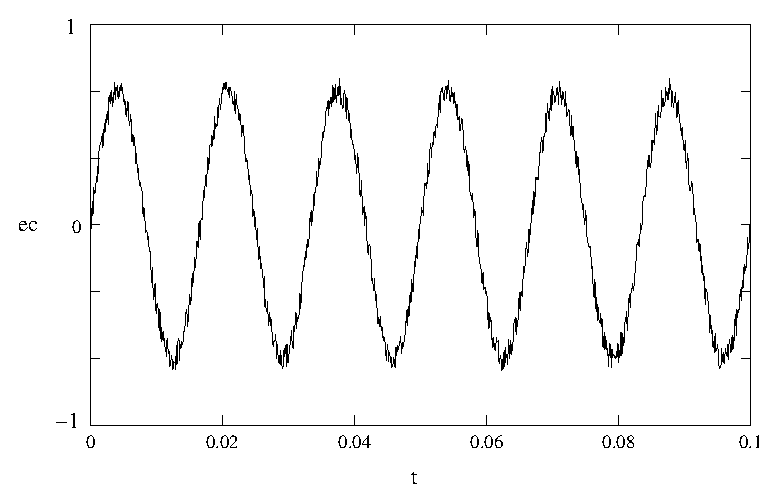
\includegraphics[width=\textwidth]{ec-sim.eps}
    \caption{$e_c(t)$ simulation.}
    \label{fig:ec-sim}
\end{center}
\end{figure}

Figure~\vref{fig:ec-sim} describes the normalized common mode signal
$e_c$. The common mode signal is consists of a 50~Hz interference
signal and a random white noise signal $e_{white}$
\begin{equation} \label{eq:ec-sim}
	e_c(t) = A_{int}\sin\/(2\pi\/f_{int}\/t) + A_{white}(2rand(t)-1) 
\end{equation}

$A_{int}$ is the amplitude of the sinusoidal interference signal. The
$rand()$ function output is scaled symmetrically around zero and
weighted to approximately 10\% of the sinusoidal amplitude. The noise
signal represents wide band interference from sources like fluorescent
lights and high--power electrical equipment.


\section{SME measurements and characterization}

This section discusses the SME implementation and presents time and
spectrum graphs of all the sinusoidal signal generators used in the
standard measurement environment. Because component tolerances exist
the measured output signal does not correspond 100\% with the
calculated design value. This is more prevalent for the
higher--frequency sources. A explanation for this phenomenon might be
the fact that a low mean resistance value for the light--bulb was
used.

\subsection{$\delta$ source measurements}

\begin{figure}[htbp]
\begin{center}
	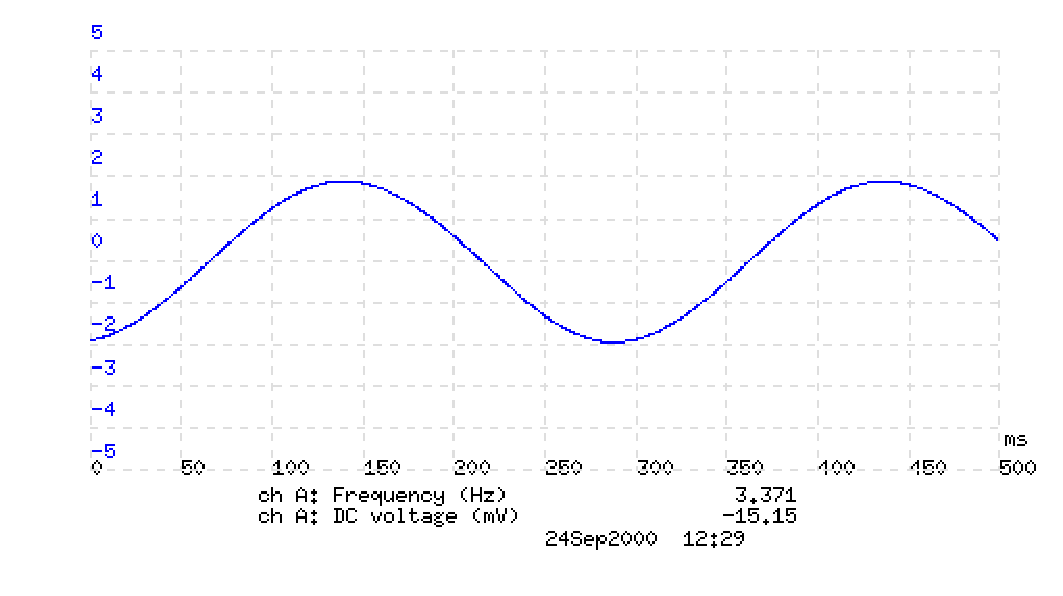
\includegraphics[width=\textwidth]{SME31.ps}
    \caption{SME 3~Hz ($\delta$) source time signal [V/ms]}
    \label{fig:sme3-1}
\end{center}
\end{figure}

Figure~\ref{fig:sme3-1} is a [V/time] trace as measured from the
output of the 3~Hz~($\delta$) SME sinusoidal signal generator. The
Y--axis represents volts. The realized $\delta$ frequency is 3.4~Hz
with a peak--to--peak amplitude of 3.78~V. A small -15.15~mV DC offset
is present. The measured frequency differs by $\pm$0.4~Hz from the
design value.

\begin{figure}[htbp]
\begin{center}
	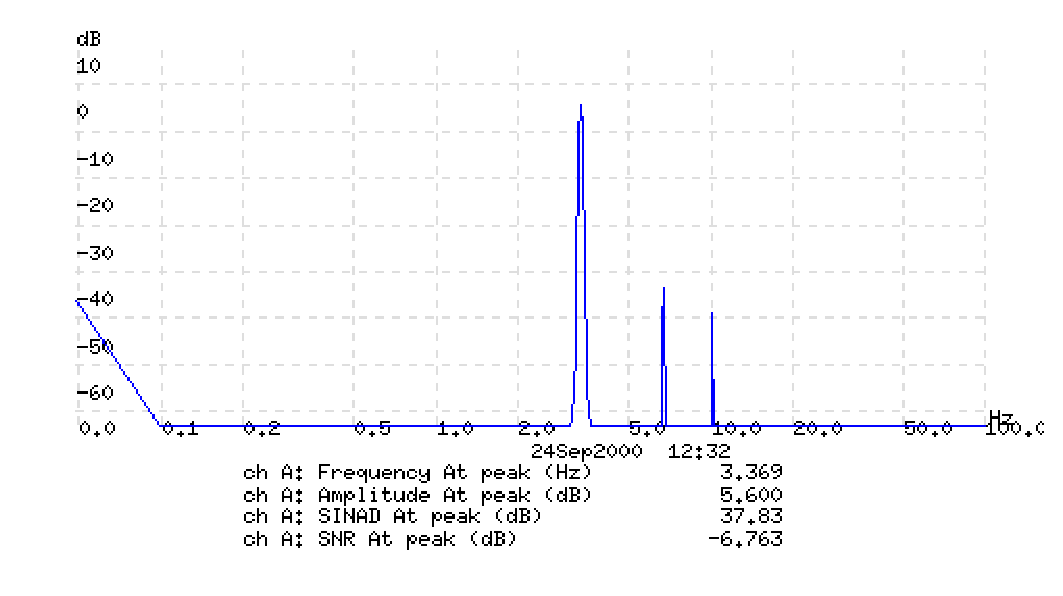
\includegraphics[width=\textwidth]{SME32.ps}
    \caption{SME 3~Hz ($\delta$) source spectrum [dB/Hz]}
    \label{fig:sme3-2}
\end{center}
\end{figure}

Figure~\ref{fig:sme3-2} is a [Power/frequency] trace as measured from
the output of the 3~Hz~($\delta$) SME sinusoidal signal generator. The
FFT was created by the PicoScope software package available from Pico
Technology Limited\footnote{http://www.picotech.com}. PicoScope is
shipped with the ADC-42 analog to digital conversion system used
during module and system testing and development. The software uses a
1~V value as the 0~dB reference.

A 2048 sample Hanning window was used to create the trace. The two
spikes to the right represents harmonies of the 3~Hz signal. A -35~dB
spike at approximately 6~Hz and a -44~dB spike at 9~Hz. Parasitic
capacitances in the circuit layout are believed to be responsible for
these spikes. It was first believed that the spikes were artifacts of
the FFT algorithm used but all of the windowing techniques available
in PicoScope delivered similar results.

The SINAD value mentioned at the bottom of Figure~\ref{fig:sme3-2} is
a ratio in dB of the signal plus noise plus distortion values to the
noise plus distortion values at the peak frequency:


\begin{equation} 
	SINAD = \frac{\sqrt{v_{rms-datum}^2 + v_{rms-1}^2 + v_{rms-2}^2 +
	...}}{\sqrt{v_{rms-1}^2 + v_{rms-2}^2 + ...}}
\label{eq:SINAD}
\end{equation}

The SINAD value is a measure of the quality of the signal. The
37.83~dB SINAD value reported by PicoScope was used to evaluate the
quality of the test signal as it progressed through the system.

\subsection{$\theta$ source measurements}

\begin{figure}[htbp]
\begin{center}
	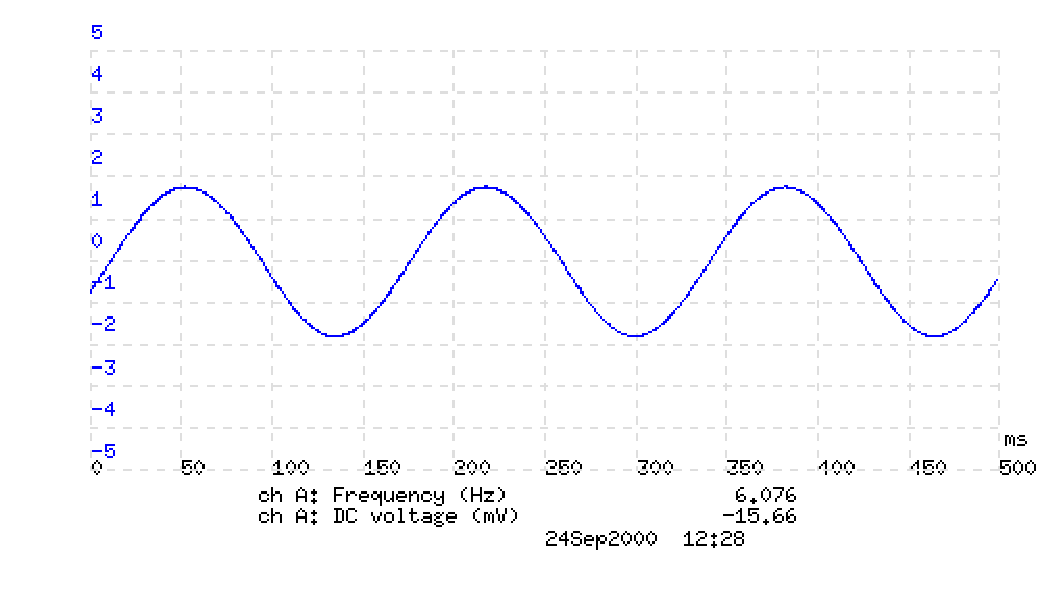
\includegraphics[width=\textwidth]{SME62.ps}
    \caption{SME 6~Hz ($\theta$) source time signal [V/time]}
    \label{fig:sme6-2}
\end{center}
\end{figure}

Figure~\ref{fig:sme6-2} is a [V/time] trace as measured from the
output of the 6~Hz~($\theta$) SME sinusoidal signal generator. The
Y--axis represents volts. The realized $\theta$ frequency is 6.1~Hz
with a peak--to--peak amplitude of 3.78~V. A small -15.66~mV DC offset
is present. The measured frequency differs by $\pm$0.1~Hz from the
design value.

\begin{figure}[htbp]
\begin{center}
	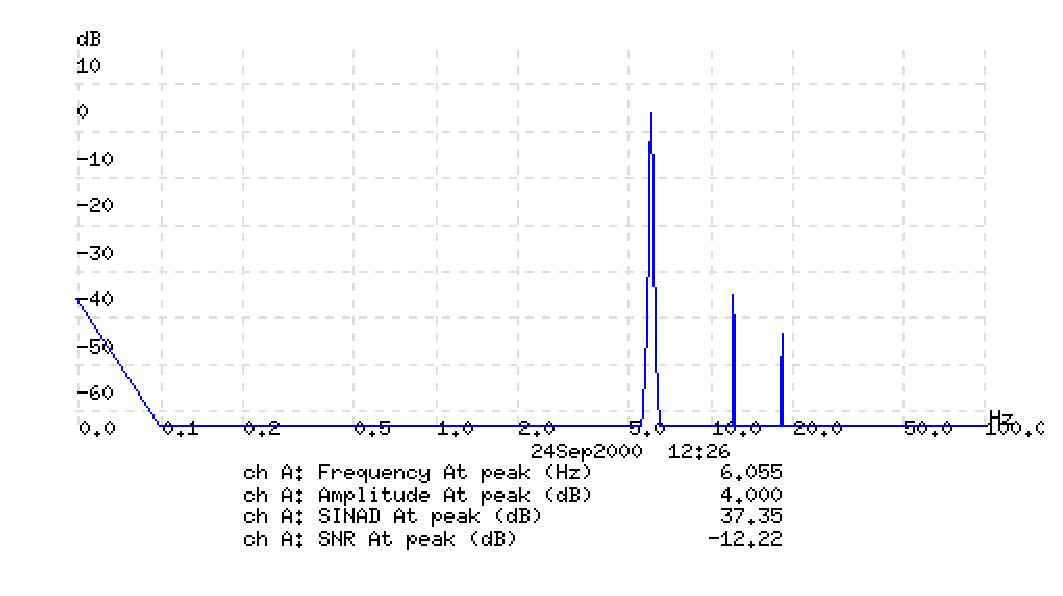
\includegraphics[width=\textwidth]{SME61.ps}
    \caption{SME 6~Hz ($\theta$) source spectrum [dB/Hz]}
    \label{fig:sme6-1}
\end{center}
\end{figure}


Figure~\ref{fig:sme6-1} is a [dB/Hz] trace as measured from the output
of the 6~Hz~($\theta$) SME sinusoidal signal generator.

A 2048 sample Hanning window was used to create the trace. The two
spikes to the right represents harmonies of the 6~Hz signal. A -35~dB
spike at approximately 12~Hz and a -45~dB spike at 18~Hz. Parasitic
capacitances in the circuit layout are believed to be responsible for
these spikes. It was first believed that the spikes were artifacts of
the FFT algorithm used but all of the windowing techniques available
in PicoScope delivered similar results.

\subsection{$\alpha$ source measurements}

\begin{figure}[htbp]
\begin{center}
	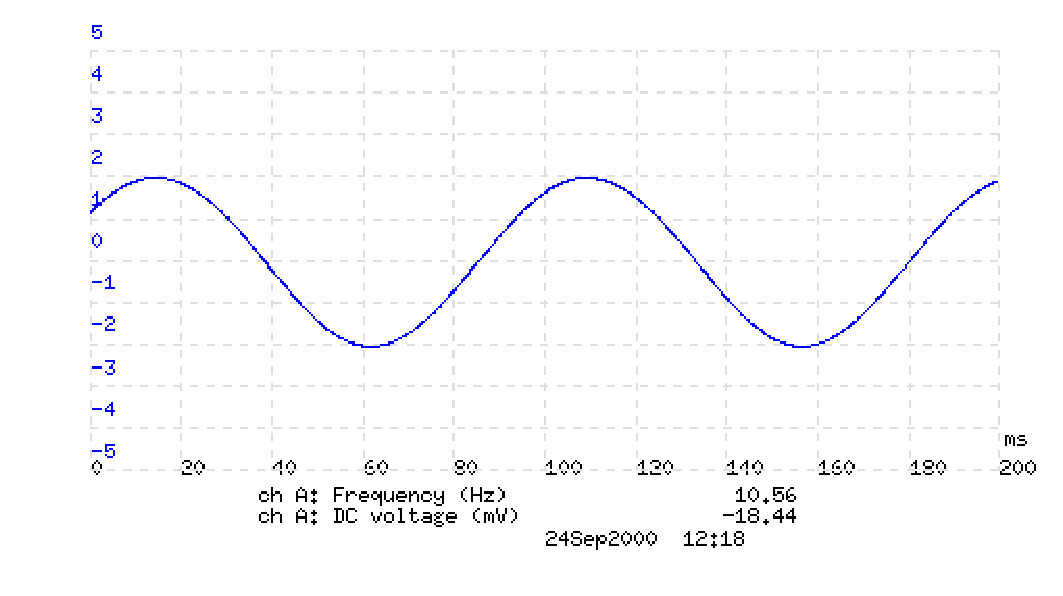
\includegraphics[width=\textwidth]{SME101.ps}
    \caption{SME 10~Hz ($\alpha$) source time signal [V/ms]}
    \label{fig:sme10-1}
\end{center}
\end{figure}

Figure~\ref{fig:sme10-1} is a [V/time] trace as measured from the
output of the 10~Hz~($\alpha$) SME sinusoidal signal generator. The
Y--axis represents volts. The realized $\alpha$ frequency is 10.5~Hz
with a peak--to--peak amplitude of 3.9~V. A small -18.44~mV DC offset
is present. The measured frequency differs by $\pm$2~Hz from the
design value.

\begin{figure}[htbp]
\begin{center}
	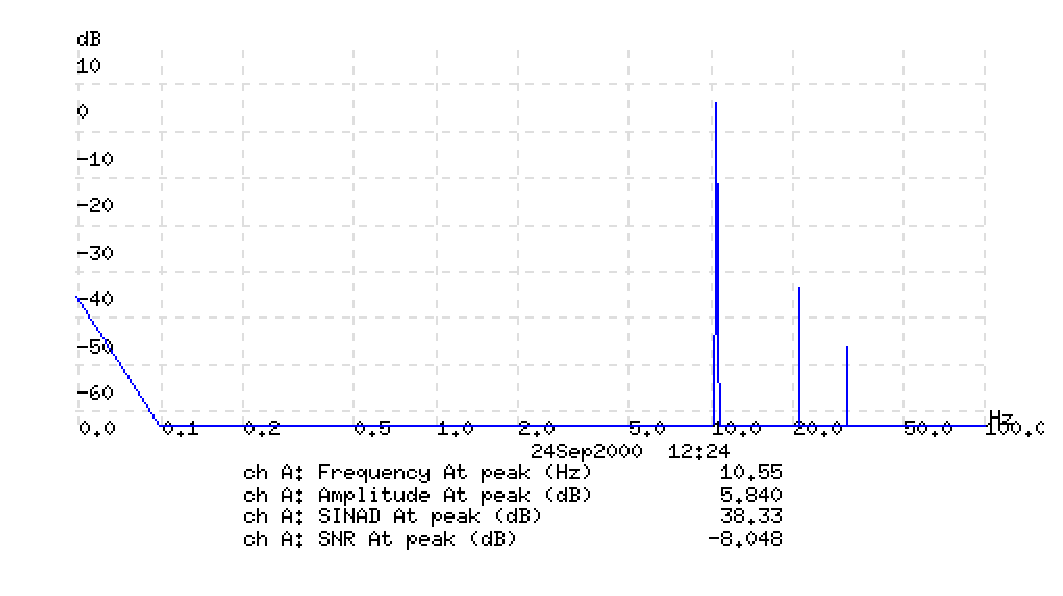
\includegraphics[width=\textwidth]{SME102.ps}
    \caption{SME 10~Hz ($\alpha$) source spectrum}
    \label{fig:sme10-2}
\end{center}
\end{figure}


Figure~\ref{fig:sme10-2} is a [Power/frequency] trace as measured from
the output of the 10~Hz~($\theta$) SME sinusoidal signal generator.

A 2048 sample Hanning window was used to create the trace. The two
spikes to the right represents harmonies of the 10~Hz signal. A -35~dB
spike at approximately 20~Hz and a -44~dB spike at 30~Hz. Parasitic
capacitances in the circuit layout are believed to be responsible for
these spikes. It was first believed that the spikes were artifacts of
the FFT algorithm used but all of the windowing techniques available
in PicoScope delivered similar results.

\subsection{$\beta$ source measurements}

\begin{figure}[htbp]
\begin{center}
	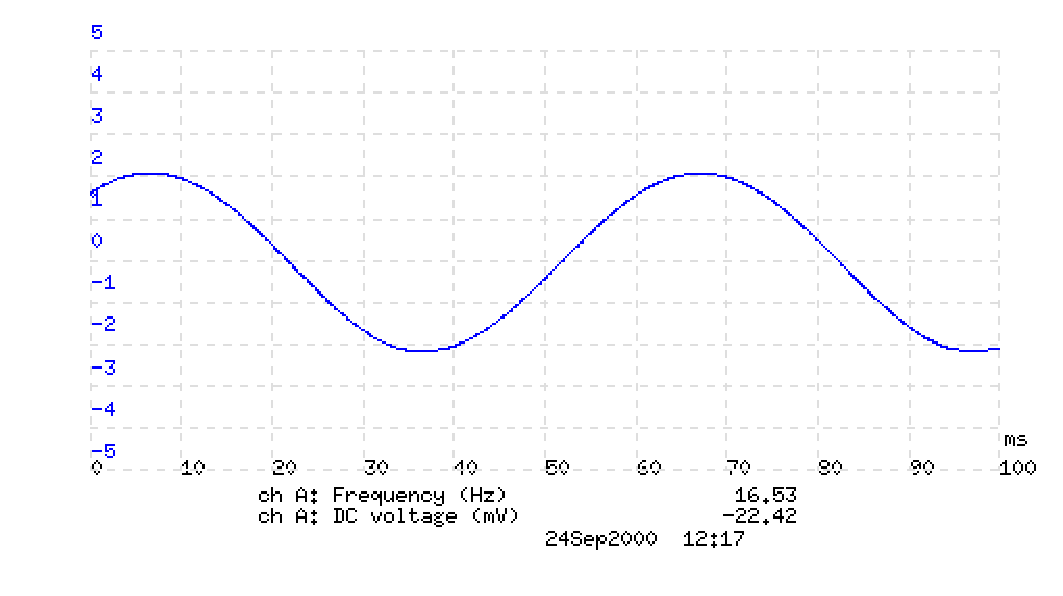
\includegraphics[width=\textwidth]{SME162.ps}
    \caption{SME 16~Hz ($\beta$) source time signal [V/time]}
    \label{fig:sme16-2}
\end{center}
\end{figure}

Figure~\ref{fig:sme16-2} is a [V/time] trace as measured from the
output of the 16~Hz~($\beta$) SME sinusoidal signal generator. The
Y--axis represents volts. The realized $\beta$ frequency is 16.5~Hz
with a peak--to--peak amplitude of 3.9~V. A small -22.42~mV DC offset
is present. The measured frequency differs by $\pm$1.5~Hz from the
design value.

\begin{figure}[htbp]
\begin{center}
	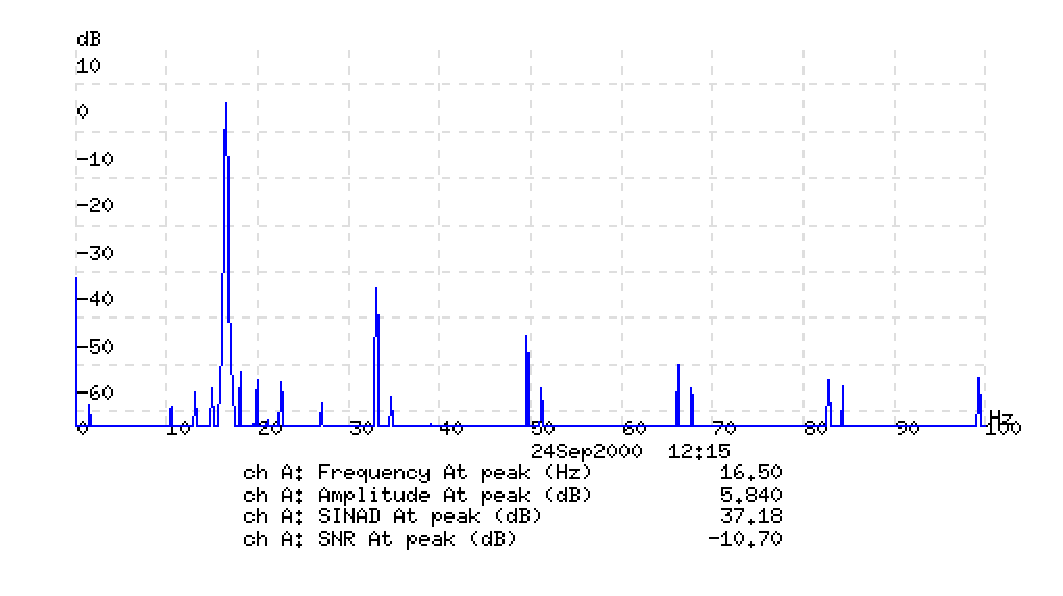
\includegraphics[width=\textwidth]{SME161.ps}
    \caption{SME 16~Hz ($\beta$) source spectrum}
    \label{fig:sme16-1}
\end{center}
\end{figure}

Figure~\ref{fig:sme16-1} is a [Power/frequency] trace as measured from
the output of the 16~Hz~($\beta$) SME sinusoidal signal generator.

A 1024 sample Hanning window was used to create the trace. The spikes
to the right represents harmonies of the 16~Hz signal. A -35~dB spike
at approximately 32~Hz and a -44~dB spike at 64~Hz are the higher
power harmonies. Parasitic capacitances in the circuit layout are
believed to be responsible for the high power spikes. The low power
spikes surrounding the base frequency and harmonies are artifacts of
the FFT algorithm used and a function of the width of the Hanning
window. In this case the window was chosen as 1024 samples, half that
of the previous measurements. Increasing the width of the window
increases the spectrum resolution and reduces algorithm artifacts at a
cost of increased computing time.


\subsection{$\gamma$ source measurements}

\begin{figure}[htbp]
\begin{center}
	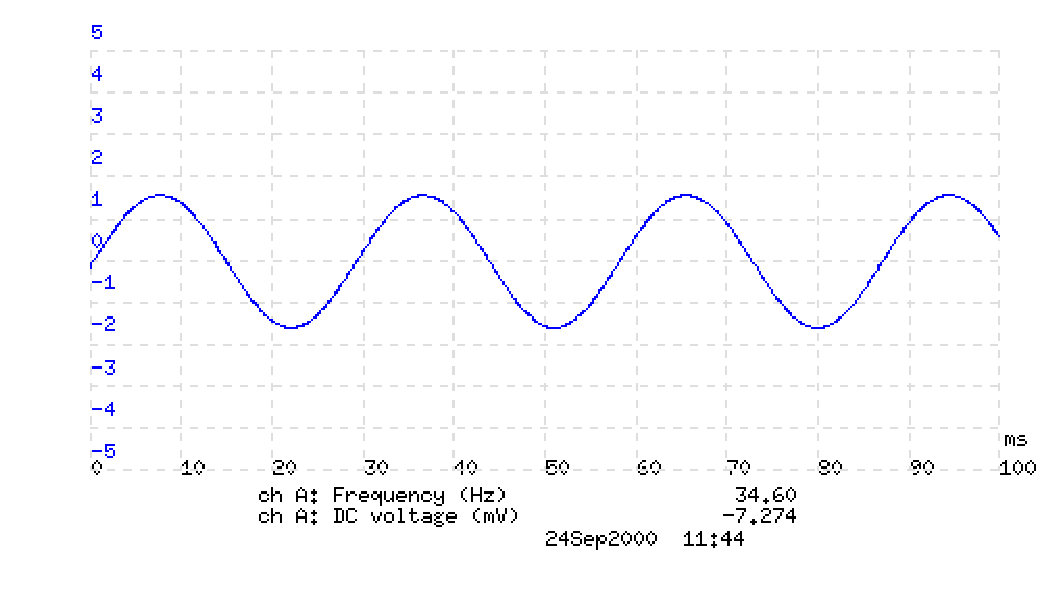
\includegraphics[width=\textwidth]{SME352.ps}
    \caption{SME 35~Hz ($\gamma$) source time signal [V/time]}
    \label{fig:sme35-2}
\end{center}
\end{figure}

Figure~\ref{fig:sme35-2} is a [V/time] trace as measured from the
output of the 35~Hz~($\gamma$) SME sinusoidal signal generator. The
Y--axis represents volts. The realized $\gamma$ frequency is 34.6~Hz
with a peak--to--peak amplitude of 3.6~V. A small -7.44~mV DC offset
is present. The measured frequency differs by $\pm$4.6~Hz from the
design value.


\begin{figure}[htbp]
\begin{center}
	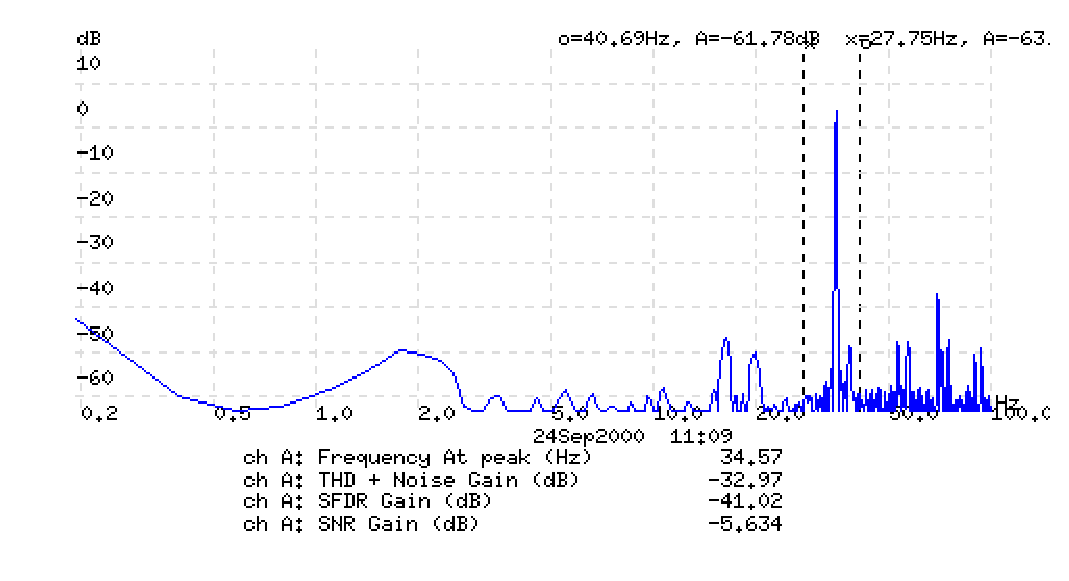
\includegraphics[width=\textwidth]{SME351.ps}
    \caption{SME 35~Hz ($\gamma$) source spectrum [dB/Hz]}
    \label{fig:sme35-1}
\end{center}
\end{figure}

Figure~\ref{fig:sme35-1} is a [dB/frequency] trace as measured from
the output of the 35~Hz~($\gamma$) SME sinusoidal signal generator.

A 1024 sample Hanning window was used to create the trace. The large
spike to the right (A -35~dB spike at approximately 70~Hz) is the
first multiple of the 35~Hz signal. Parasitic capacitances in the
circuit layout are believed to be responsible for the high power
spikes. The low power spikes surrounding the base frequency and
harmonies are artifacts of the FFT algorithm used and a function of
the width of the Hanning window. In this case the window was chosen as
1024 samples, half that of the previous measurements. Increasing the
width of the window increases the spectrum resolution and reduces
algorithm artifacts at a cost of computing time.


\begin{figure}[htbp]
\begin{center}
	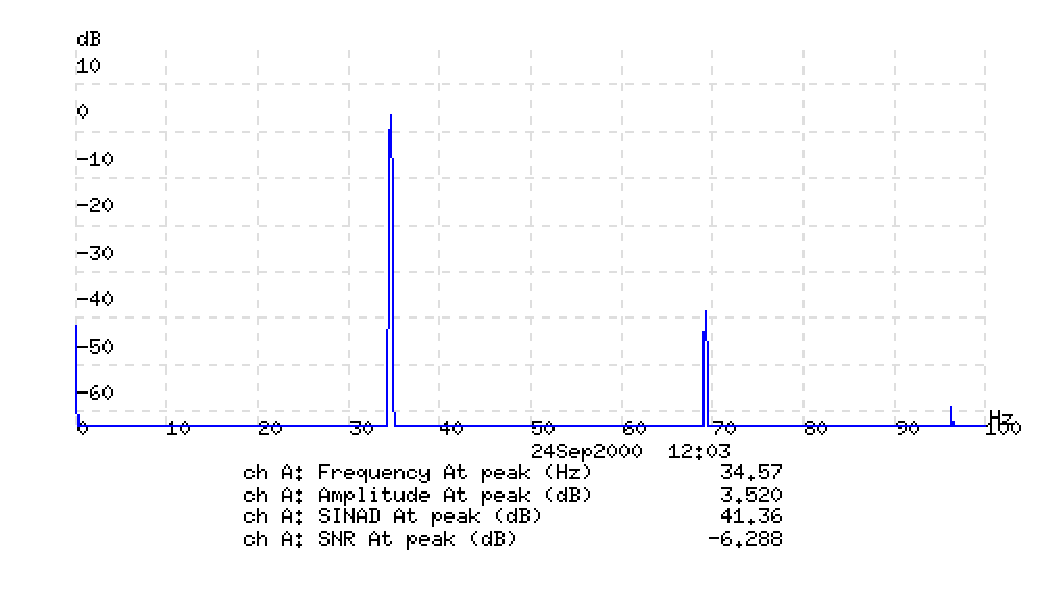
\includegraphics[width=\textwidth]{SME353.ps}
    \caption{SME 35~Hz $\gamma$ source spectrum [dB/Hz], 4096 Hanning window}
    \label{fig:sme35-3}
\end{center}
\end{figure}

Figure~\ref{fig:sme35-3} is reproduced as it illustrates a important
caveat when dealing with digital Fourier Transform (DFT)
implementations and their various algorithms. Figure~\ref{fig:sme35-3}
represents exactly the same signal as that of
Figure~\ref{fig:sme35-1}. The difference in representations are a
result of the width of the Hanning window used in creating the
result. Figure~\ref{fig:sme35-3} was created using a 4096 sample width
Hanning window, Figure~\ref{fig:sme35-1} used a 1024 width
window. Visual inspection of both graphs would imply that
Figure~\ref{fig:sme35-1} is more 'noisy' than
Figure~\ref{fig:sme35-3}, this assumption is false and may lead to a
incorrect interpretation of the signal trace.

\section{General Testing procedure} \label{section:test-proc}

The $\alpha$ signal from Table~\ref{table:test-pros} is used as the
standard test signal throughout the implementation of a specific
module. When it was deemed necessary other test frequencies were also
used. All test signals used were chosen from the signals specified in
Table~\ref{table:test-pros} and implemented using the Wein--bridge
oscillators previously discussed.


